\documentclass[aspectratio=1610]{beamer}
%\linespread{1.5}\selectfont

\usepackage{booktabs}
\usepackage{dcolumn}
\usepackage{float}
\usepackage{placeins}
\usepackage{lscape} 
\usepackage{tikz}
\usepackage[export]{adjustbox}
\usepackage{ragged2e}
\justifying
\usepackage{outlines}
\usepackage{amsmath}
\usepackage{booktabs}
\usepackage{float}
\usepackage{dcolumn}
\usepackage{longtable}
\usepackage{array}
\usepackage{multirow}
\usepackage{wrapfig}
\usepackage{float}
\usepackage{colortbl}
\usepackage{pdflscape}
\usepackage{tabu}
\usepackage{threeparttable}
\usepackage{caption}
%\captionsetup{font=footnotesize}
\usepackage{subcaption}
\usepackage{threeparttable}
\usepackage[normalem]{ulem}
\usepackage{makecell}
\usepackage{xcolor}
\usepackage{hyperref}
\hypersetup{colorlinks = true, linkcolor = red, urlcolor = teal, citecolor = blue}

%\usepackage{caption}
%\captionsetup{labelformat=empty}
\usepackage{appendixnumberbeamer}

\DeclareUnicodeCharacter{2212}{-}
\DeclareUnicodeCharacter{0327}{\c}

\usepackage[backend = biber, style=authoryear, sorting = nty, maxnames=1]{biblatex}

\addbibresource{citations_sesmarias.bib}

%\addbibresource[location = remote]{https://raw.githubusercontent.com/ViniOkadaSilva/Papers/master/Sesmarias/citations_sesmarias.bib}

\DeclareFieldFormat{citehyperref}{%
  \DeclareFieldAlias{bibhyperref}{noformat}% Avoid nested links
  \bibhyperref{#1}}

\DeclareFieldFormat{textcitehyperref}{%
  \DeclareFieldAlias{bibhyperref}{noformat}% Avoid nested links
  \bibhyperref{%
    #1%
    \ifbool{cbx:parens}
      {\bibcloseparen\global\boolfalse{cbx:parens}}
      {}}}

\savebibmacro{cite}
\savebibmacro{textcite}

\renewbibmacro*{cite}{%
  \printtext[citehyperref]{%
    \restorebibmacro{cite}%
    \usebibmacro{cite}}}

\renewbibmacro*{textcite}{%
  \ifboolexpr{
    ( not test {\iffieldundef{prenote}} and
      test {\ifnumequal{\value{citecount}}{1}} )
    or
    ( not test {\iffieldundef{postnote}} and
      test {\ifnumequal{\value{citecount}}{\value{citetotal}}} )
  }
    {\DeclareFieldAlias{textcitehyperref}{noformat}}
    {}%
  \printtext[textcitehyperref]{%
    \restorebibmacro{textcite}%
    \usebibmacro{textcite}}}

\renewcommand*{\nameyeardelim}{\addcomma\space}

\usepackage{setspace}

\DeclareUnicodeCharacter{0301}{\'{e}}
\usepackage{graphicx}

\newcommand{\tinytable}[1]{\textcolor{black}{\tiny \input{#1}}}

\graphicspath{{~/OneDrive - University of Illinois - Urbana/Research/Writing/git/Sesmarias/Pictures/}}

\beamertemplatenavigationsymbolsempty

%Information to be included in the title page:
\title{Sesmaria Land Grants and the Origins of Brazilian Inequality}
\author{Vinicius Okada da Silva}
\institute{The University of Illinois at Urbana-Champaign}
\date{}

\setbeamertemplate{footline}[frame number]

\begin{document}


\begin{frame}[plain, noframenumbering]
	\titlepage
\end{frame}

\begin{frame}{History}
    \begin{outline}
        \1 Originally a medieval Portuguese Law used to grant lands to be used and developed.
        \1 First mention of it in Brazil was in 1530, and it often favored the Portuguese aristocracy \parencite{Lobb1976-mc}
            \2 Early studies argued it led to the development of the ``economic aristocracy of the colonial society'' and the ``principal cause of the \textit{latifundio}'' in Brazil \parencites[p.~36]{Lima2002-kd}[p.~48]{Da_Costa_Porto1979-dz}.
            \2 Officially stopped being granted in 1822 with Brazil's independence \cite{Silva2019-vj}. 
            \2 However, effectively, land grants in Brazil came under a new regime in 1850 with the \textit{Lei das Terras} [ADD CITATION].
            \2 However, \textit{sesmeiros} who had owned land and had developed it would be able to retain their lands. 
    \end{outline}    
\end{frame}

\begin{frame}{Research Question}
    \begin{outline}
        \1 What are the long-term economic effects of the \textit{sesmarias} land grants in Brazil?
            \2 Land inequality $\Rightarrow$ only those with financial conditions were granted \textit{sesmarias}, and were often granted large plots of land.
            \2 Income inequality $\Rightarrow$ land was wealth, fewer people with land lead to wealth accumulation by the few.
            %\2 Urban development $\Rightarrow$ .
    \end{outline}
\end{frame}

\begin{frame}{Data}
    \begin{outline}
        \1 Brazilian Censuses (1872-2010)
        \1 Location of \textit{sesmarias} from \href{http://plataformasilb.cchla.ufrn.br/}{SILB}.
    \end{outline}
\end{frame}

\begin{frame}{Example of Document}
    \begin{figure}
        \centering
        \begin{subfigure}[t]{0.35\textwidth}
        \centering
        \vspace{-7.4cm}
        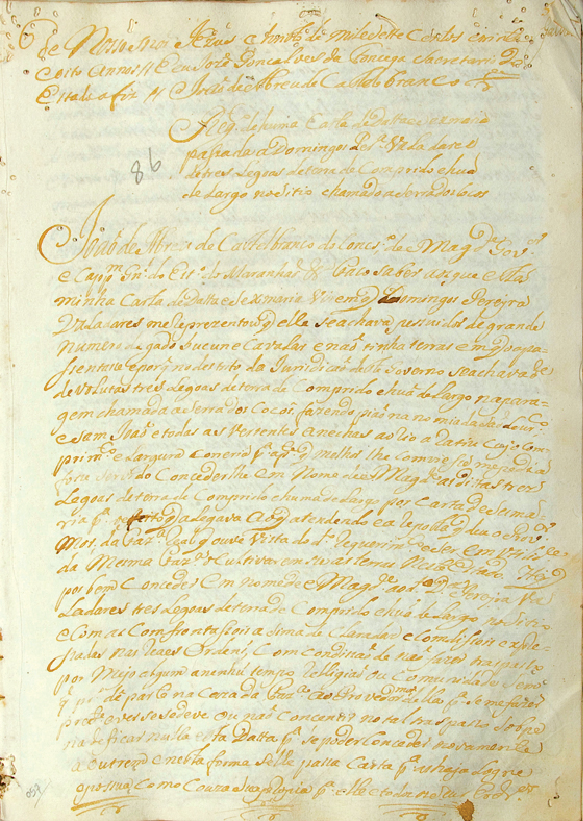
\includegraphics[width = \textwidth]
        {0167f614a7c3b3fd38127f1545dbee7c.pdf}
        \end{subfigure}
        \hspace{0.2cm}
        \qquad\tikz[baseline=-\baselineskip]\draw[ultra thick,->] (0,4) -- ++ (1,0);\qquad
        \hspace{-0.25cm}
        \begin{subfigure}[t]{0.4\textwidth}
        \centering
        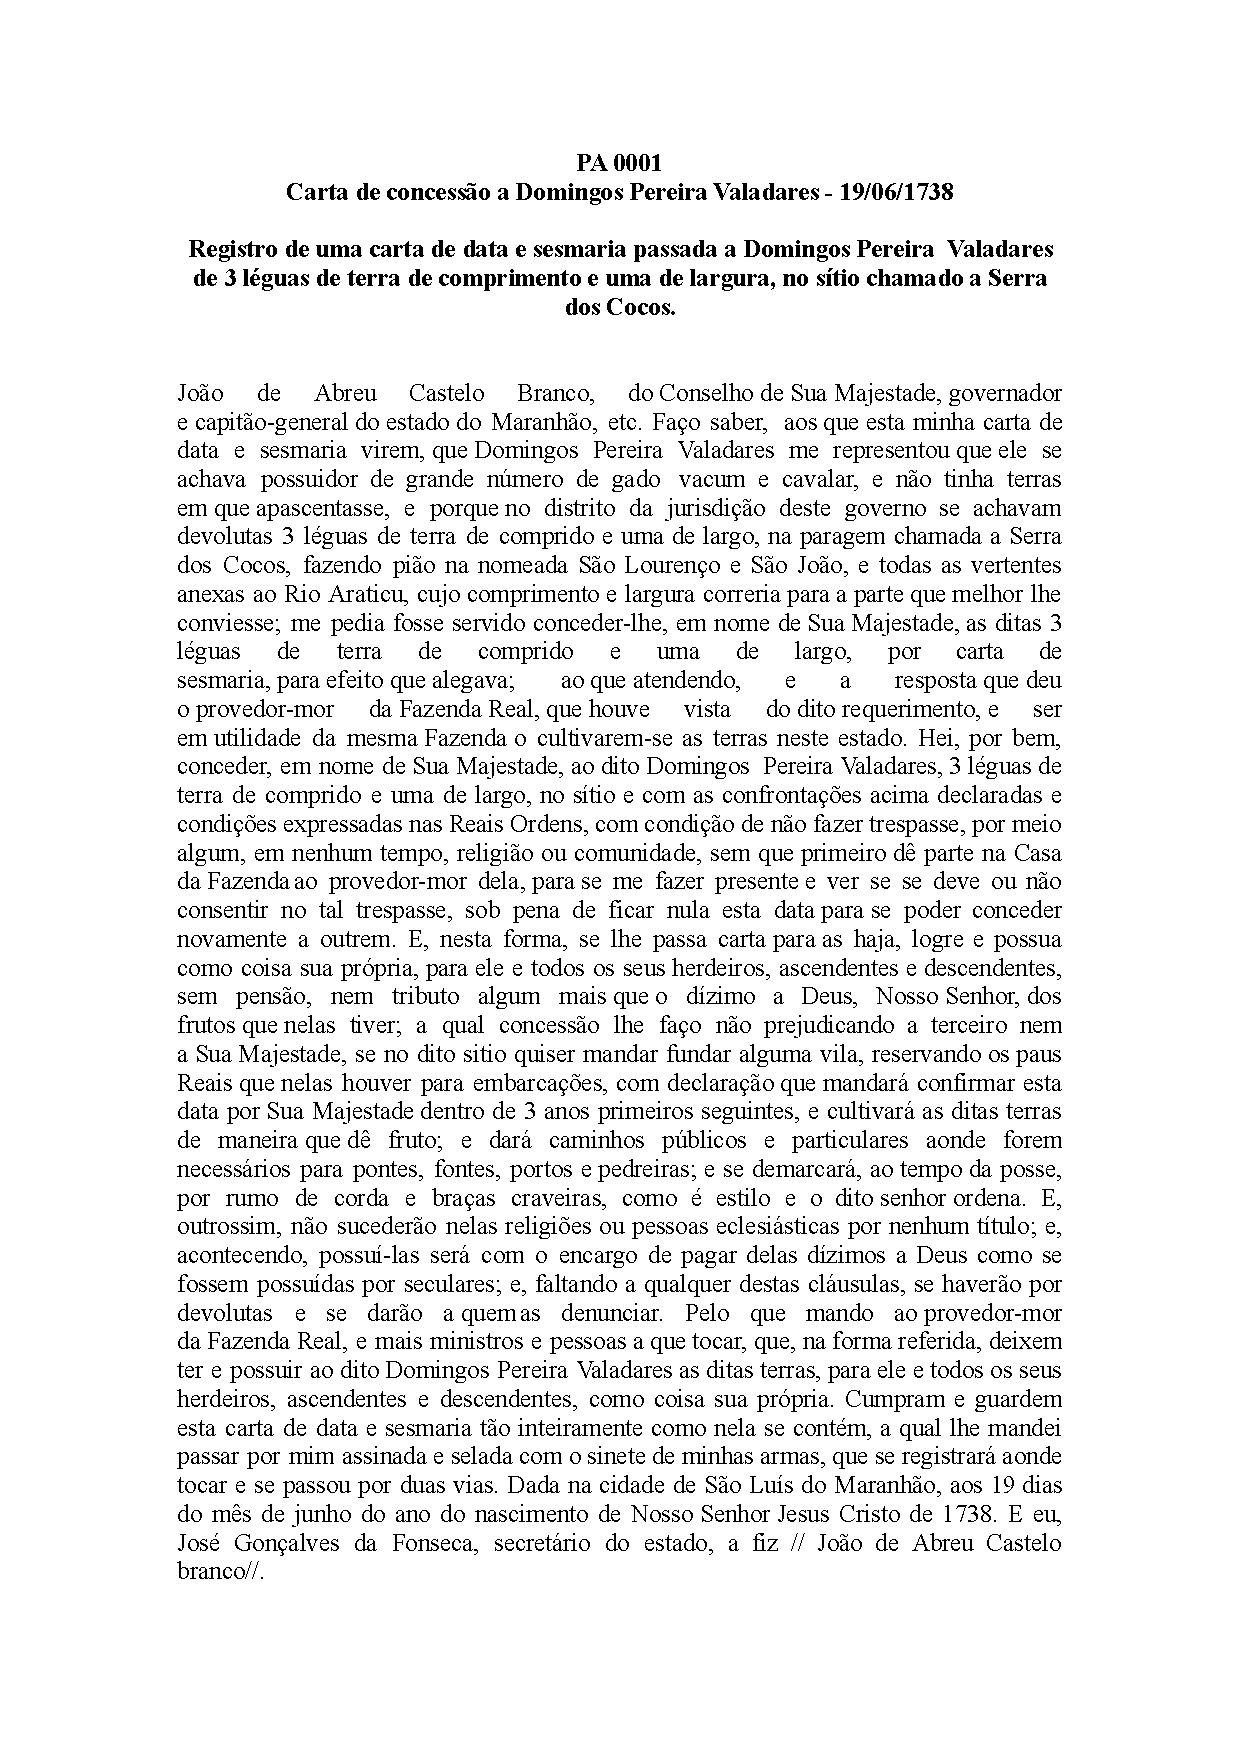
\includegraphics[page = 1, width = \textwidth]
        {ea71ea6ac7c5ec3cefa24ded60ac6438.pdf}
        \end{subfigure}
    \end{figure}
\end{frame}

\begin{frame}{Possible Sources of Variation}
    \begin{outline}
        \1 Geographical Variation
        \1 Time Variation
        \1 Type of Settler to whom it was granted
        \1 Concessions vs. Applications
        \1 What purpose was the land requested (production of cows, sugar plantation, etc.)
    \end{outline}
\end{frame}

\begin{frame}{Other possibilities?}
    \begin{outline}
        \1 Possible to focus only where we would expect them to have an effect and spend time transcribing/focusing on them.
            \2 ``Under the auspices of King Philip I (1581-1598), the sesmaria was widely applied in the northeast and central coast regions of Brazil where a system involving large properties and slave labor was considered the only way to make a profit in the new land, whether by means of cultivation or cattle ranching.''\parencite{Lobb1976-mc}
            \2 Sugarcane plantations required extensive amounts of slave labor \parencite{Silva2019-vj}
    \end{outline}
\end{frame}

\begin{frame}{Other Relevant (?) Information to Add}
    \begin{outline}
        \1 Sesmarias caused land uncertainty in colonial times as often poor people would settle, develop land, and then lose the right of the land because a richer person would claim it \parencite[p.~142]{Da_Costa_Porto1979-dz}.
    \end{outline}
\end{frame}

\begin{frame}[allowframebreaks, t]{References}
    \printbibliography
\end{frame}

\end{document}